\documentclass[12pt]{article}
\usepackage[utf8]{inputenc}
\usepackage[T1]{fontenc}
\usepackage{pdflscape} 
\usepackage{lmodern}
\usepackage{amsmath}
\usepackage[a4paper,bindingoffset=0.2in,%
            left=0.5in,right=0.5in,top=0.5in,bottom=1in,%
            footskip=.25in]{geometry}
\usepackage[colorlinks=true, linkcolor=Black, urlcolor=Blue]{hyperref}
\usepackage{graphicx}
\usepackage{subcaption}
\usepackage{listings}
\usepackage{color}
\usepackage{float}
\usepackage[usenames, dvipsnames]{xcolor}

\definecolor{codegreen}{rgb}{0,0.6,0}
\definecolor{codegray}{rgb}{0.5,0.5,0.5}
\definecolor{codepurple}{rgb}{0.58,0,0.82}
\definecolor{backcolour}{rgb}{0.95,0.95,0.92}

\lstdefinestyle{mystyle}{
	backgroundcolor=\color{backcolour},   
	commentstyle=\color{codegreen},
	keywordstyle=\color{magenta},
	numberstyle=\tiny\color{codegray},
	stringstyle=\color{codepurple},
	basicstyle=\ttfamily\footnotesize,
	breakatwhitespace=false,         
	breaklines=true,                 
	captionpos=b,                    
	keepspaces=true,                 
	numbers=left,                    
	numbersep=5pt,                  
	showspaces=false,                
	showstringspaces=false,
	showtabs=false,                  
	tabsize=2
}


\begin{document}
\title{Projekt 2: Analiza możliwości algorytmów optymalizacji\\
\large Sebastian Michoń 136770, Marcin Zatorski 136834\\
\large grupa L5}
\date{\vspace{-10ex}}
\maketitle

\section{Zarys idei}
\begin{enumerate}
	\item Obliczenia przeprowadzano dla 2 architekur:
	\begin{enumerate}
		\item Standardowa sieć neuronowa, złożona z warstw gęstych o kolejno 10-50-100-100-100-5 neuronach (10 neuronów wejściowych, 5 wyjściowych).
	\end{enumerate}
	\item Porównanie optymalizatorów było elementem hiperparameter tuningu i badania wpływu poszczególnych metod regularyzacji na poszczególne optymalizatory.
	\item Operacje przeporwadzone dla pierwszej architektury:
	\begin{enumerate}
		\item Stworzono pewną sieć neuronową, dane treningowe i dane testowe. Dane treningowe składały się z 50.000 instancji, dane testowe z 10.000 instancji (instancje składały się z 10 wartości).
		\item Uruchamiano losowo zainicjalizowaną (z biasem z rozkładu normalnego i wagami pochodzącymi z jednorodnego inicjalizatora Xaviera) sieć neuronową dla danych treningowych. Będzie ona nazywana dalej prewzorcową siecią neuronową.
		\item W każdym pojedynczym eksperymencie porównywano określone optymalizatory w następujący sposób:
		\begin{enumerate}
			\item Ustalano ground truth jako rezultat propagacji zestawu treningowego i testowego przez sieć neuronową z wagami pochodzącymi z prewzorcowej sieci neuronowej i regularyzacją (gdyby używać prewzorcowej sieci neuronowej z takimi samymi wagami i bez regularyzacji, wyniki mogłyby się różnić dla regularyzacji 'batch  normalization'; Dzięki rozwiązaniu zadania w taki sposób spełniono założenie o identycznej architekturze sieci neuronowych jednocześnie - dzięki kopiowaniu wag - umożliwiając porównywanie rezultatów dla różnych rodzajów regularyzacji). Sieć ta nazywana będzie wzorcową siecią neuronową.
			\item Tworzono sieć neuronową dla podanej metody regularyzacji i podanych hiperparametrów (np. dropout\_rate=0.2). Nazywana ona będzie dalej testową sięcią neuronową
			\item Trenowano testową sieć neuronową w 3 epokach.
			\item Po wytrenowaniu testowej sieci neuronowej ewaluowano ją na zbiorze treningowym, testowym i porównywano wagi w dwóch sieciach neuronowych: testowej i wzorcowej.
		\end{enumerate}
	\end{enumerate}
	\item Funkcją kosztu dla porównania danych wyjściowych było MSE.
	\item Dla pierwszej architektury eksperymenty przeprowadzono dla następujących typów regularyzacji:
	\begin{enumerate}
		\item \textbf{batch\_normalization}: przeprowadzano testy dla 3 optymalizatorów: SGD, Adam i AdamW(weight\_decay = 0.0001). Przeprowadzono testy dla każdej pary złożonej z wartości z ciągu [4, 16, 64, 256] dla parametru batch\_size i wartości z ciągu [0.1, 0.5, 0.9, 0.95, 0.99, 0.999] dla parametru momentum - w sumie wykonano 24 testy dla tej regularyzacji.
		
		\item \textbf{weight\_decay}: przeprowadzano testy dla 2 optymalizatorów: SGDW i AdamW. Przeprowadzono testy dla każdej wartości z ciągu [0.5, 0.1, 0.01, 0.001, 0.0001, 0.00001] dla parametru weight\_decay - w sumie wykonano 6 testów dla tej regularyzacji.
		
		\item \textbf{dropout}: przeprowadzano testy dla 3 optymalizatorów: SGD, Adam i AdamW(weight\_decay = 0.0001). Przeprowadzono testy dla każdej wartości z ciągu [0, 0.1, 0.2, 0.3, 0.4, 0.5] dla parametru dropout\_rate - w sumie wykonano 6 testów dla tej regularyzacji.
	\end{enumerate}
	Wykonano zatem w sumie 36 testów. Wartwy Dropout / Batch normalization wstawiono pomiędzy każdą parę warstw gęstych z wyłączeniem pierwszych 2 warstw (czyli na przykład 10-50-Dropout-100-Dropout-100-Dropout-100-Dropout-5).
	
	
	\item \label{tit:cost} Funkcja kosztu wag:
	\begin{enumerate}
		\item Zaimplementowano standardową funkcję liczącą MSE będącą uśrednioną sumą błędów kwadratowych dla wszystkich wag i biasów (bias liczony był w średniej jako jedna z wag).
		\item Aby porównywać wagi neuronów, które są w jakiś sposób związane, przed wyliczeniem funkcji kosztu modyfikowano macierze wag w wytrenowanej testowej sieci neuronowej tak, aby neurony, które mają podobne wartości wag i biasa na wejściu były na tych samych pozycjach w obydwu porównywanych sieciach neuronowych.
		\item W \textit{tensorflow} element macierzy wag $W_{i,j}$ oznacza wagę $i$-tego wyjścia z poprzedniej warstwy dla $j$-tego wejścia kolejnej warstwy. Co za tym idzie, wektor $V_j=[W_{1,j}, W_{2,j} \dots W_{n,j}, b_j]$ reprezentuje kolejne wagi na wejściu $j$-tego neurona w kolejnej warstwie.
		\item Dla wszystkich macierzy wag i biasów - począwszy od pierwszej - porównywano ujemne podobieństwo kosinusowe pomiędzy każdą parą wektorów $V_j$ w obu sieciach (wzorcowej i testowej) dla tej samej warstwy.
		\item Celem metody była maksymalizacja podobieństwa neuronów na tych samych pozycjach; w tym celu wykorzystano metodę węgierską, aby wybrać minimalną możliwą sumę ujemnych podobieństw kosinusowych przy pewnej zamianie miejscami pozycji neuronów. Rezultatem metody węgierskiej była sekwencja par $1:a_1, 2:a_2, \dots m:a_m$ oznaczająca, że aby zminimalizować sumę ujemnych podobieństw kosinusowych wektorów wag (z biasem) dla pojedynczego neurona należy dokonać takiej transformacji na macierzy wag, aby kolumna o indeksie $a_i$ była na pozycji \(i\)-tej po transformacji testowej sieci neuronowej. Transormację tę osiągnięto przez:
		$$\begin{bmatrix}
			k_1 & k_2 \dots k_m\\
		\end{bmatrix}
		\begin{bmatrix}
			e_{a_1} & e_{a_2} & \dots e_{a_m}\\
		\end{bmatrix}
		=
		\begin{bmatrix}
			k'_1 & k'_2 & \dots k'_m\\
		\end{bmatrix}
		$$
		gdzie \(e_i\) oznacza pionowy wektor jednostkowy o wypełniony zerami i jedną jedynką w pozycji \(i\)-tej, wektory jednostkowe mają rozmiar \(m\) (macierz z prawej jest kwadratowa), wektory \(k_j\) to kolumny macierzy wag przed transformacją. W ten sam sposób transformowano wektor biasów.
		\item Analogicznie, jeśli za daną warstwą była inna wartswa gęsta, zamieniono kolejnością wiersze następnej macierzy wag tak, aby kolejność neuronów była taka sama w obu macierzach (a zatem należało zmienić kolejność wartości wychodzących z poprzedniej warstwy):
		$$\begin{bmatrix}
			e_{a_1}^T\\ e_{a_2}^T\\ \dots\\ e_{a_m}^T\\
		\end{bmatrix}
		\begin{bmatrix}
			w_1\\ w_2\\ \dots\\ w_m\\
		\end{bmatrix}
		=
		\begin{bmatrix}
			w'_1\\ w'_2\\ \dots\\ w'_m\\
		\end{bmatrix}
		$$ gdzie $w_i$ oznacza $i$-ty wiersz pierwotnej macierzy. Nie transformowano wektora biasów, ponieważ nie miał on związku z transformacją pozycji wyjść z poprzedniej warstwy.
	\end{enumerate}
\end{enumerate}
\section{Rezultaty i ich omówienie}
\subsection{Testy pierwszej sieci}
\subsubsection{Testy batch normalization}
\begin{figure}[h!]
	\centering
	\begin{subfigure}[b]{1\linewidth}
		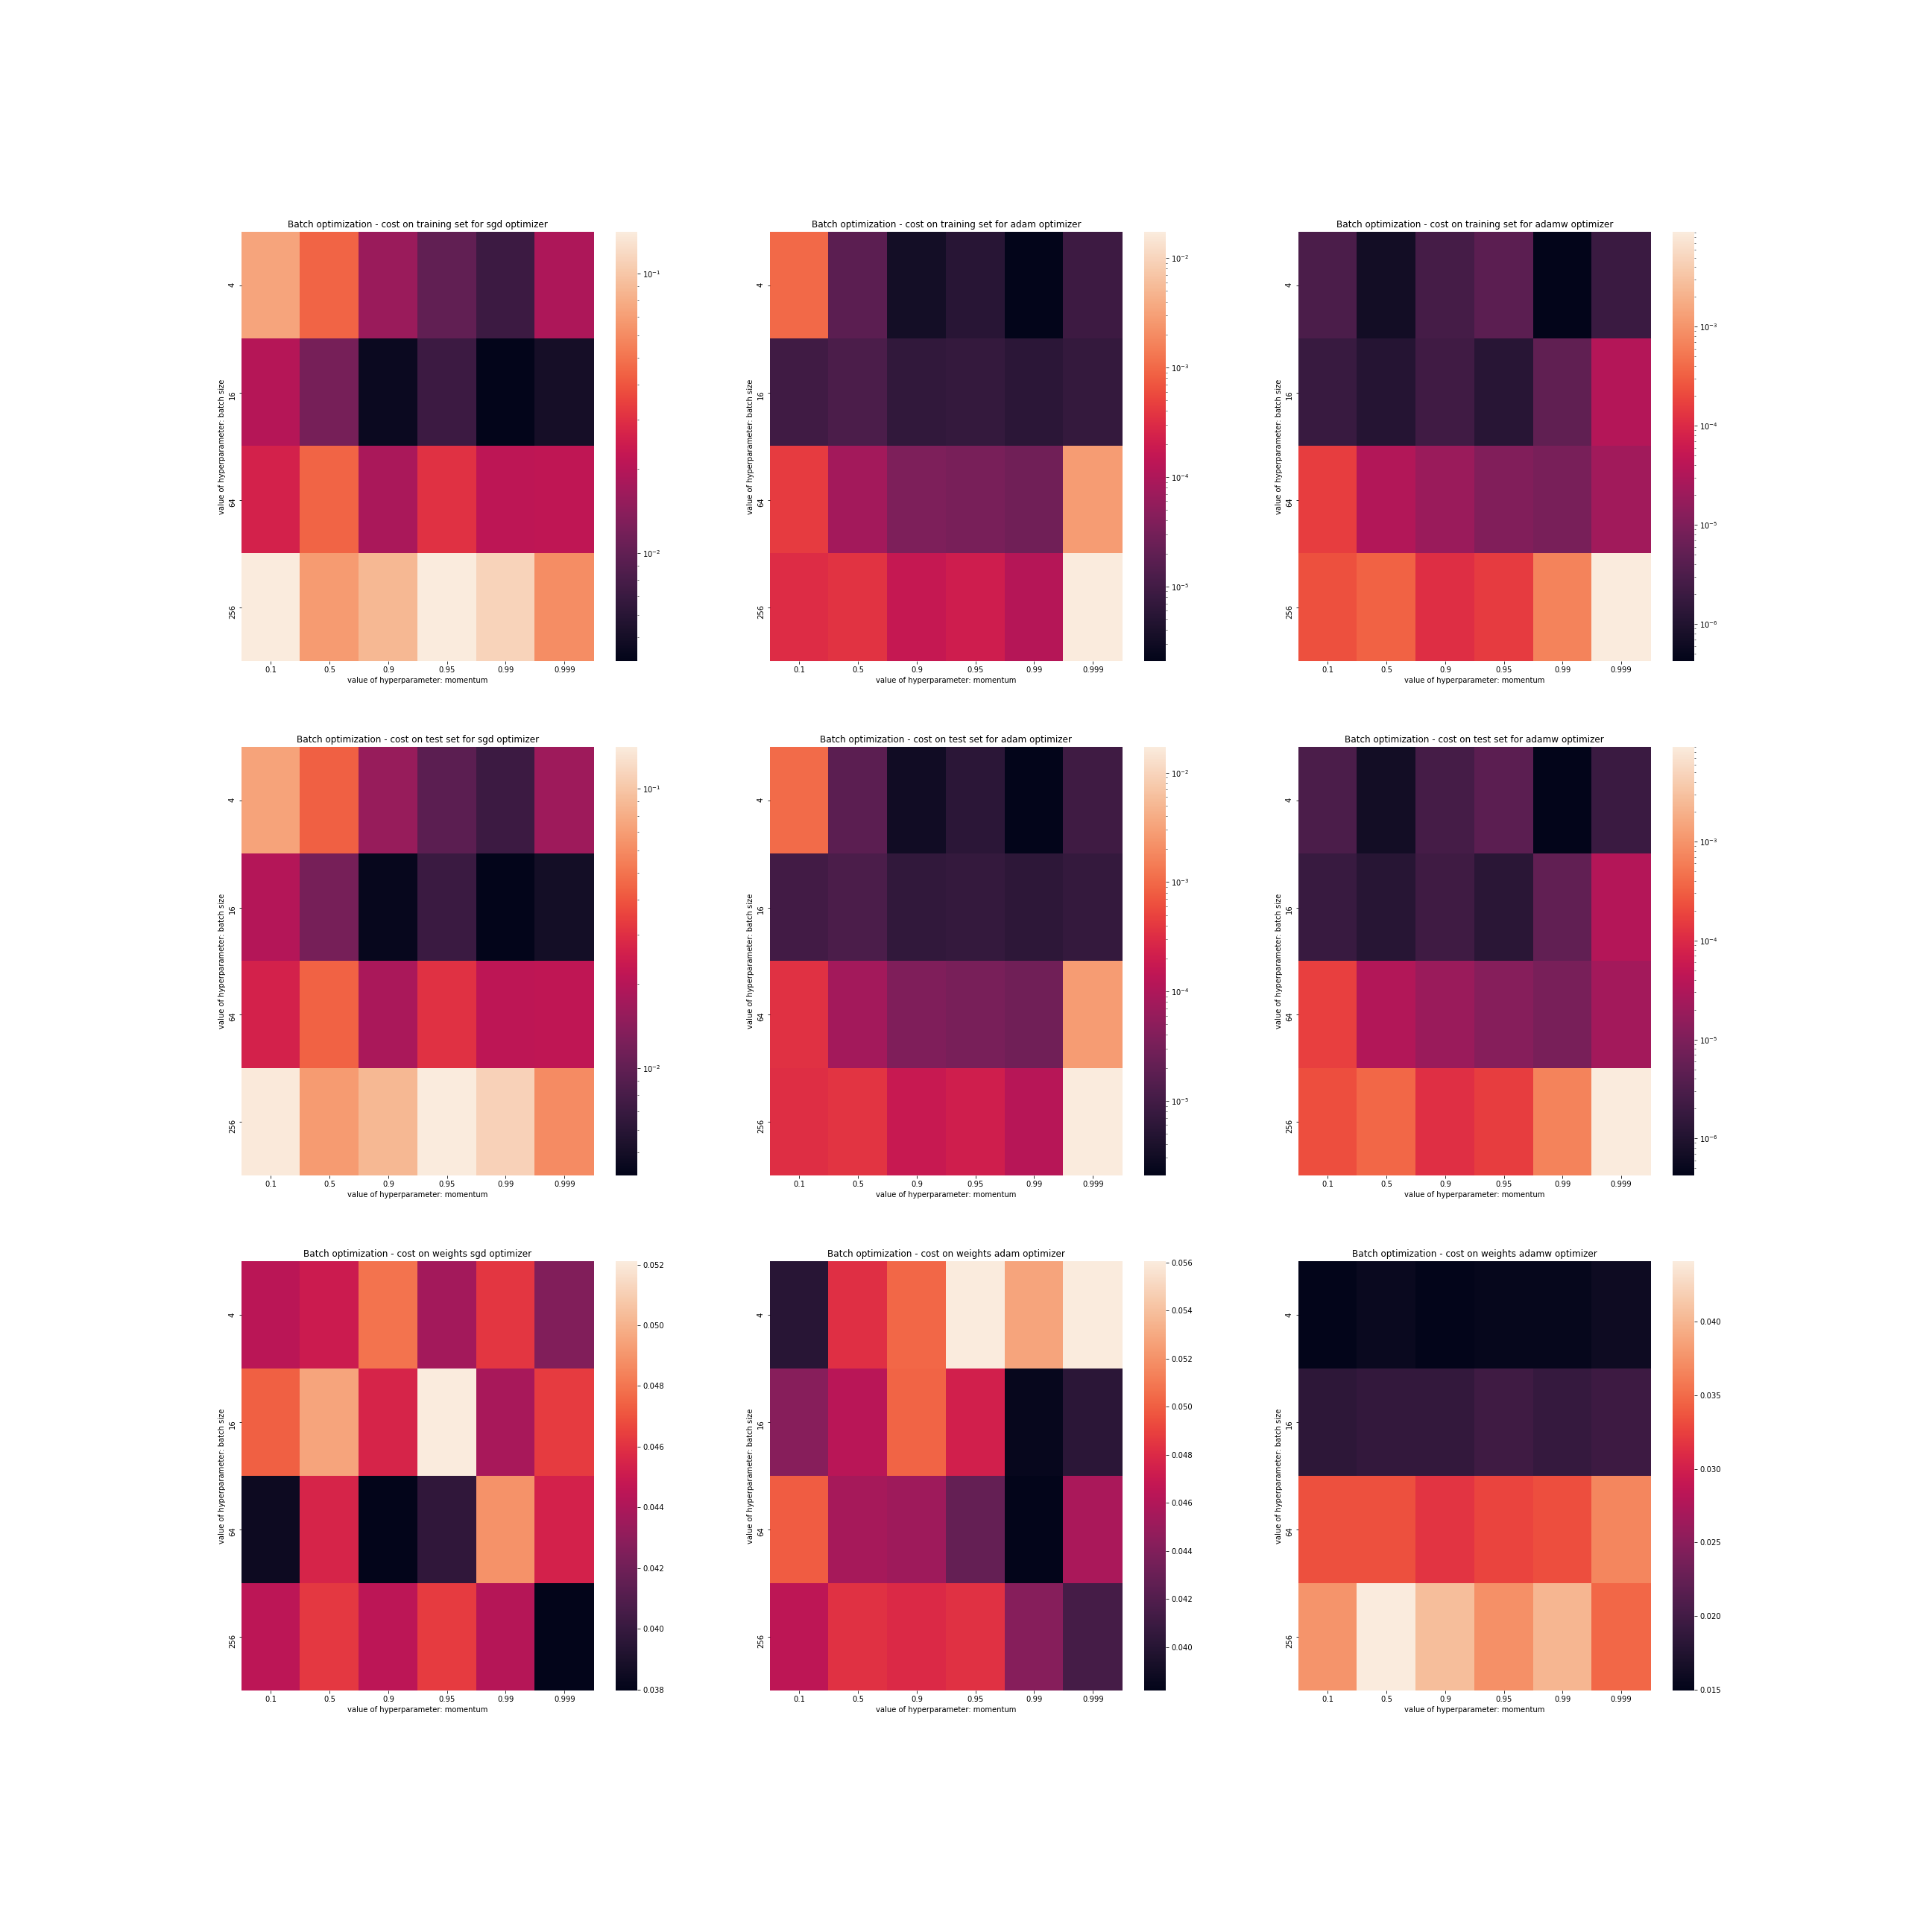
\includegraphics[width=\linewidth]{Comparision_batch_norm.png}
	\end{subfigure}
	\label{fig:batch}
	\caption{Rezultaty nauki sieci z regularyzacją typu batch normalization}
\end{figure}
Opis testów i ich rezultatów:
\begin{enumerate}
	\item Na tym i każdym kolejnym wykresie wartości funkcji kosztu dla zestawu testowego i treningowego będą przedstawiane w skali logarytmicznej, nawet dla SGD.
	\item Wartości funckji kosztu dla zbioru treningowego i testowego są nieomal identyczne - wynika to z:
	\begin{enumerate}
		\item 50.000 Instancji danych treningowych pochodzących z tego samego rozkładu - pociąga to za sobą możliwość efektywnego wytrenowania sieci.
		\item Braku szumu w danych wyjściowych - Wzorcowe wartości na wyjściu są funkcją zależną jedynie od inputu.
		\item Identycznej architektury obu sieci neuronowych.
	\end{enumerate}
	Obserwacja ta będzie zauważalna we wszystkich kolejnych testach.
	\item Najlepsze rezultaty optymalizacji SGD (wartość MSE rzędu około 0.01) są porównywalne z najgorszymi rezultatami optymalizacji Adam i AdamW. Obserwacja ta będzie się powtarzała w kolejnych testach.
	\item Wszystkie optymalizatory uzyskały najniższe wartości funkcji kosztu dla momentum=0.99.
	\item Dla SGD najlepsze wyniki osiągano dla batch\_size=16, dla Adam i AdamW dla batch\_size=4.
	\item Wartości fukcji kosztu dla batch\_size wyższego równego 64 są prawie zawsze wyższe niż dla mniejszego batch\_size.
	\item AdamW dla batch\_size=4 bardzo dobrze dopasowywał się do wag sieci wzorcowej; żaden inny optymalizator nie osiągnął podobnych rezultatów dla opisanej w paragrafie \ref{tit:cost} funckji kosztu (0.15 AdamW względem 0.38 SGD i Adama). W ogólności Adam\_W lepiej dopasowywał wagi do sieci wzorcowej niż pozostałe optymalizatory.
	\item Dla wartości funckji kosztu osiąganej przez optymalizaotry Adam i AdamW niemożliwość perfekcyjnego dopasowania do wzorcowej sieci neuronowej może wynikać między innymi z błędów zaokrągleń.
\end{enumerate}

\subsubsection{Testy weight decay}
\begin{figure}[H]
	\centering
	\begin{subfigure}[b]{1\linewidth}
		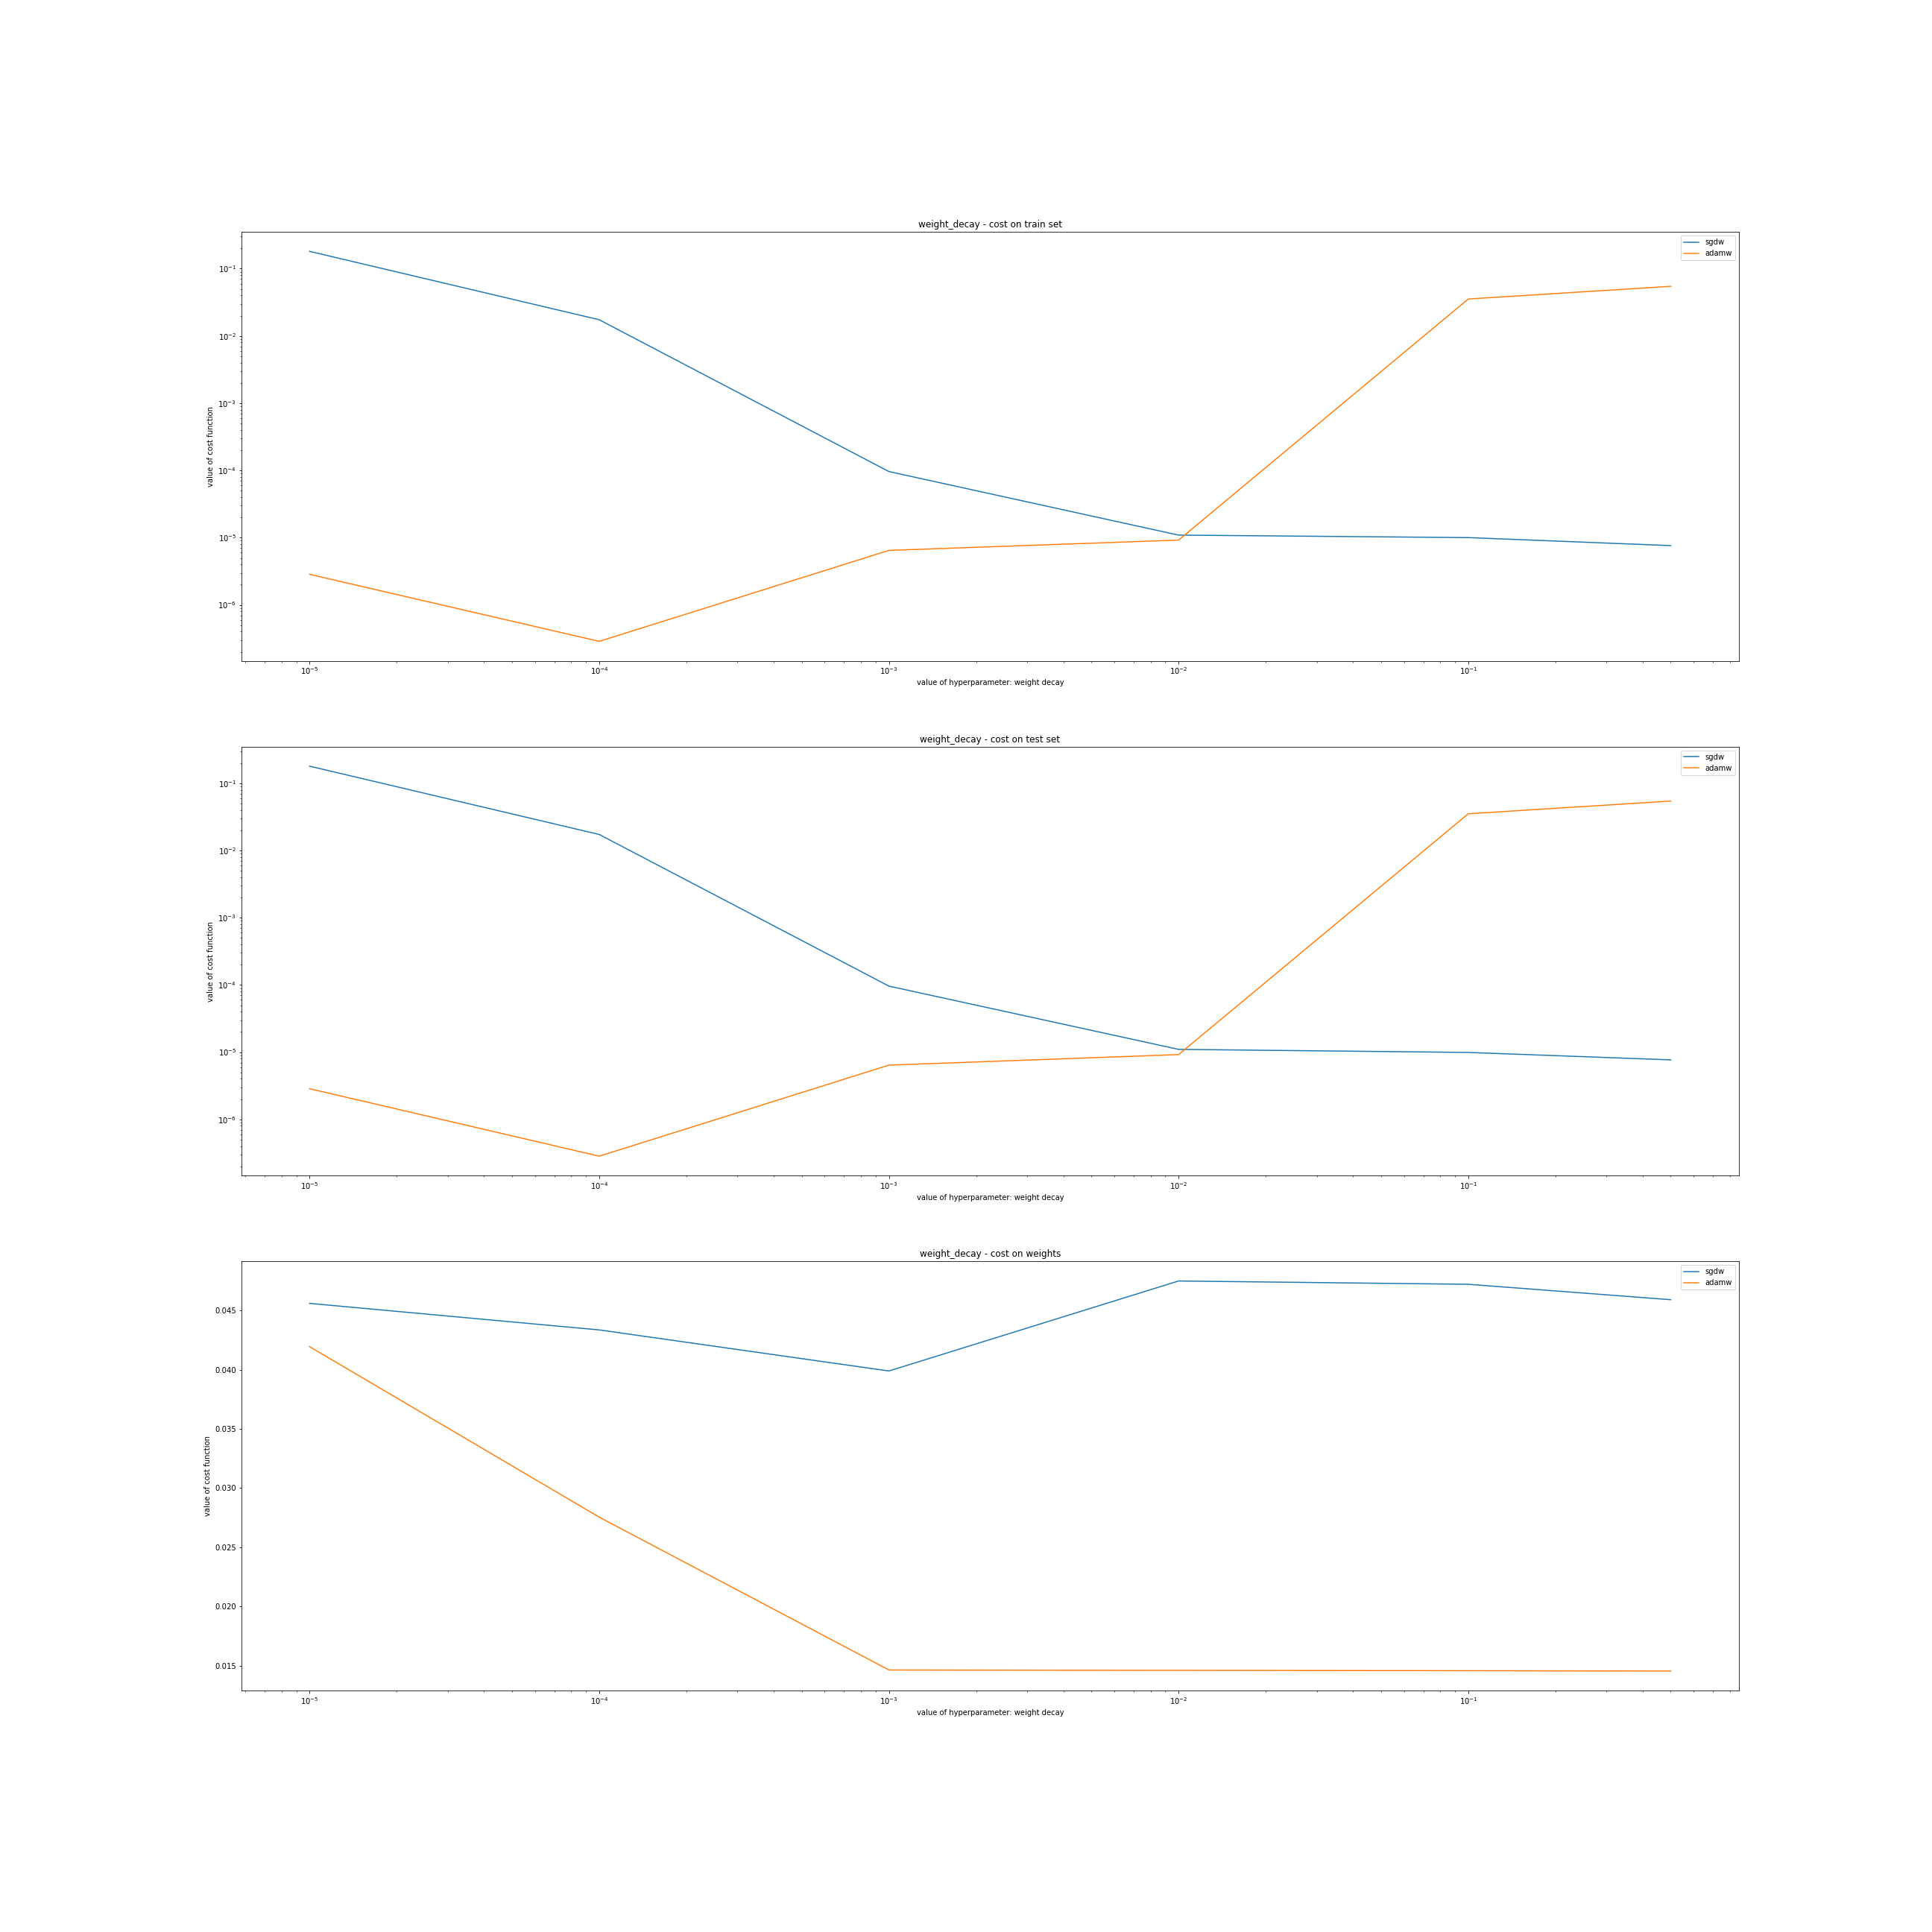
\includegraphics[width=\linewidth]{Comparision_weight_decay.png}
	\end{subfigure}
	\label{fig:decay}
	\caption{Rezultaty nauki sieci z róznymi wartościami weight decay w optymalizatorze.}
\end{figure}
Opis testów i ich rezultatów:
\begin{enumerate}
	\item Skale na obu osiach są skalami logarytmicznymi z wyjątkiem ostatniego rysunku, gdzie na osi y jest skala liniowa.
	\item Optymalizator SGDW osiągał najlepsze rezlutaty dla weight decay większego niż 0.1, z kolei AdamW osiągał najlepsze rezultaty dla weight decay rzędu \(10^{-4}\).
	\item Pomimo ponad stukrotnie wyższej wartości funkcji kosztu dla zestawu testowego i treningowego dla AdamW niż SGDW dla weight decay rzędu 0.1, funkcja kosztu dla wag była około 3 razy niższa dla algorytmu AdamW niż dla SGDW. W ogólności, funkcja kosztu wag była prawie stała dla SGDW (na poziomie 0.45) i malejąca dla AdamW.
	\item Najlepsze rezultaty osiągane przez SGDW i AdamW są podobne (około 10 razy niższe dla AdamW), co pokazuje wyższą skuteczność optymlizatora SGDW z odpowiednio dobraną wagą niż standardowego optymalizatora SGD.
\end{enumerate}

\subsubsection{Testy dropoutu}
\begin{figure}[H]
	\centering
	\begin{subfigure}[b]{1\linewidth}
		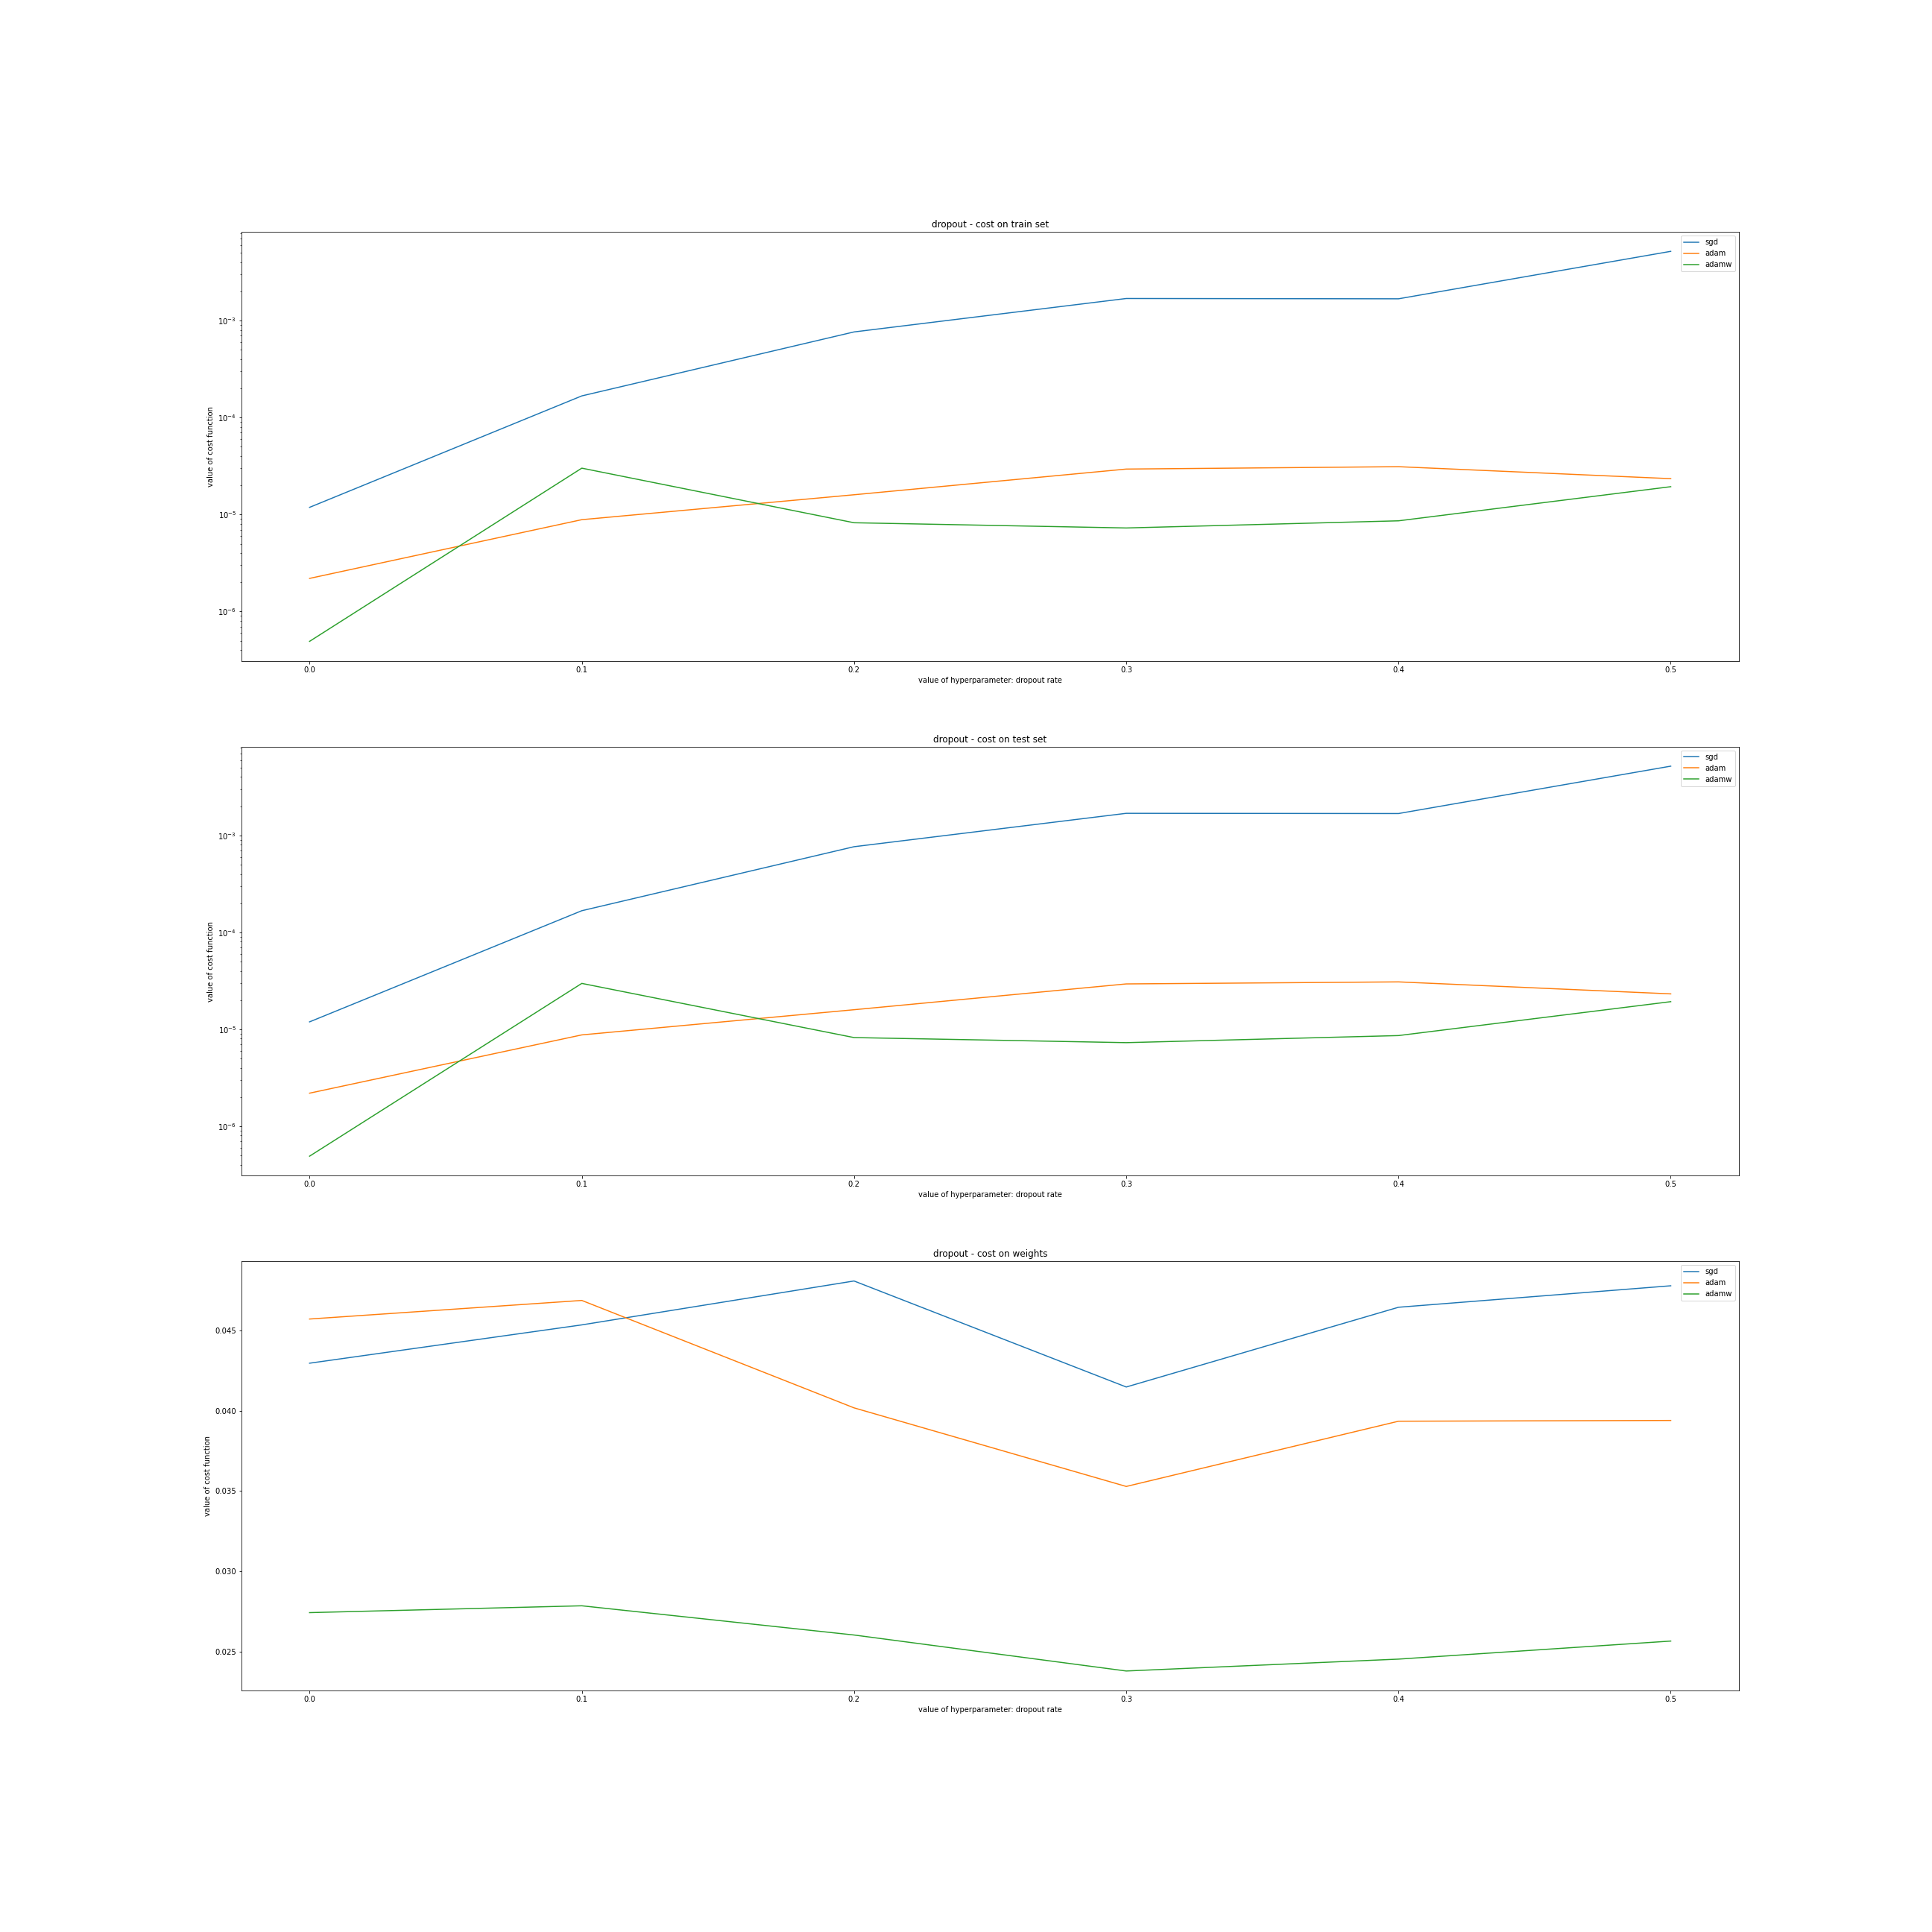
\includegraphics[width=\linewidth]{Comparision_dropout.png}
	\end{subfigure}
	\caption{Rezultaty nauki sieci z róznymi wartościami weight decay w optymalizatorze.}
	\label{fig:dropout}
\end{figure}
Opis testów i ich rezultatów:
\begin{enumerate}
	\item Skale na osi y są skalami logarytmicznymi z wyjątkiem ostatniego rysunku, gdzie na osi y jest skala liniowa.
	\item Wzrost dropout rate często prowadził do wyższych wartości funkcji kosztu na zestawach treningowym i testowym - może to wynikać z kilku czynników:
	\begin{enumerate}
		\item Celem dodania dropoutu jest uniknięcie przetrenowania i dostosowania się sieci neuronowej do wyników obarczonym pewnym szumem; w tych danych nie ma żadnego szumu, teoretycznie można osiągnąć funkcję kosztu równą 0 dla każdych danych.
		\item Istnienie dropoutu może penalizować próbę upodobnienia sieci testowej do wzorcowej sieci neuronowej, np. przez odrzucanie neuronów istniejących we wzorcowej sieci mających kluczowy wpływ na rezultat.
	\end{enumerate}
	\item Wszystkie 3 optymalizatory osiągały najbardziej podobną sieć neuronową do sieci wzrocowej dla dropout\_rate=0.3.
\end{enumerate}
\subsubsection{Uwagi ogólne}
\begin{enumerate}
	\item Optymalizator SGD osiągał gorsze rezultaty na zbiorach treningowym i testowym z normalizacją niż bez niej. Jego najlepszy rezultat to $MSE \approx 10^{-5}$, dla Adama ta wartość wynosiła $MSE \approx 2*10^{-6}$, a dla AdamW $MSE \approx 5*10^{-7}$. \item Regularyzacja prowadziła do zmniejszenia funkcji kosztu wag, co można zauważyć na wykresie \ref{fig:dropout} (pokazującym funkcję kosztu wag w zależności od dropoutu).
\end{enumerate}

\clearpage

\section{Wnioski}
\begin{enumerate}
	\item Optymalizator SGD zawsze osiągał gorsze rezultaty niż AdamW z weight\_decay=$10^{-4}$, ponadto nie wykonywał się szybciej niż AdamW.
	\item Wykorzystanie optymalizatora AdamW z dobrze dopasowanym weight\_decay praktycznie zawsze prowadzi do lepszych rezultatów niż wykorzystanie optymalizatora Adam - zarówno w kontekście podobieństwa wag sieci neuronowych, jak i funkcji kosztu.
	\item Wartość weight\_decay ma bardzo duży wpływ na działanie optymalizatora, może powodować nawet osiągnięcie nawet $10^5$ razy mniejszej funkcji kosztu niż dowolna wartość tego hiperparametru. Optymalna wartość tego hiperparametru jest zależna od algorytmu.
	\item Parametr momentum dla batch normalization na poziomie 0.99 zdaje się być odpowiedni dla testowanych optymalizatorów, taka jest też jego domyślna wartość w tensorflowie.
	\item Przy używaniu batch normalization niższa wartość batch\_size niekoniecznie prowadziła do lepszej wartości funkcji kosztu pomimo dłuższego przetwarzania i większej liczby aktualizacji wag dla tej samej liczby epok (jest to widoczne dla optymalizatora SGD).
	\item W specyficznym przypadku bez żadnego "szumu" w danych wyjściowych dropout nie prowadził do polepszenia predykcji na zbiorach treningowym i testowym, wręcz przeciwnie. Wartość dropoutu na poziomie 0.3 pozwalała natomiast najlepiej dopasować się do macierzy wag. W ogólności, w testach pierwszej architektury regularyzacja niewiele przynosiła w kontekście funkcji kosztu zarówno dla zbioru treningowego, jak i testowego.
\end{enumerate}

\end{document}
